\section{Validation}

In order to quantify the value of this \textit{tranformational} approach, a validation tools is necessary. The extraction of Partially Observable Markov Decision Processes from Simulink model is simply a transformation between different dynamic system descriptions, a transformation from a rule based system description to a probabilistic state transitional system. Ideally such a transformation would produce a perfect representation of the source model. Unfortunately different assumptions and simplifications may have a derogatory effect on the quality of the system representation. The \textit{validator} aims to help identify the qualitative shortcomings of an extraction product.

% \subsection{Motivation}

% The motivation behind the development of a Markov Process validator is that

\subsection{Approach}

The \textit{validator} measures qualitative difference between two dynamic system descriptions by comparing the responses of the two system to idential stimulation. The approach of analysing the response of a dynamic system to well-defined stimulation comes from the field on control, as this method can often provide insight into the system's behaviour. Linear time-invariant system are, for example, completely defined by their impulse response, ie. the reponse to other input signals can be deduced from the impulse response. Common stimulation signals include the Dirac Delta function, the Heaviside step function, sine functions or white noise.

This approach is based on the assumption that similar responses to identical stimulation implies similar system descriptions. Given that the \textit{extractor} simply transforms a model described in one way (Simulink) to a model described in another way (Markov Process) the response of these two systems should be similar given similar stimulation.

The difference between the responses of both systems may thus be an accurate measure of the qualitative deficit of the Markov Process description.

\subsection{Limitations}

This validation approach does have certain limitations. Mainly it is based on the assumption that similar responses imply similar system dynamics. Although this can be said of linear time-invariant systems, it may not be the case for other types of models. This must be kept in mind when assessing the quality of an extracted model. A number of other limitations exist.

Firstly the validator can only be used with single-output models. The response difference is not computed in the continuous domain, but rather in state space, meaning that the outputs of simulations of the Simulink models are mapped into the Markov Process's state space and then compared. In order to assess the variance of the two systems' responses, the state space must then be ordered. Unfortunately ordering only supports one-dimensional values (n-dimensional spaces cannot easily be ordered).

Additionaly a comparison of a continuous model with a discrete model requires the discretization of the former, meaning that the quality of the transformed model can only be judged as far as the discretization permits. Rough discretization parameters may hide some of the source model's underlying dynamics, yet still not be correctly recognized by this validation tool. The quality of its assessment is limited by the roughness of the transformation's discretization.

Finally the comparison is also limited by the conversion ratio between simulation time steps and Markov Process epochs (see section~\ref{subsec:timestepsdecisionepochs}). Because this ratio may be greater (but never less) than $1$, the dynamics of the system between epochs cannot be compared to the response of the Markov Process. This means that a comparison is only possible at every epoch, even though the original model may show significant non-linear behaviour between these time steps. The \texit{validator} can thus not provide a qualitative assessment of the differences between epochs.

\subsection{Results}
\label{subsec:validatorresults}

The \textit{validator} produces a number of outputs that can be used to judge the quality of the transformation. Firstly it produces box plots of the distribution of the systems' response in state space over time. These plots can be used to assess the variance between the responses of the two systems. Secondly it produces a plot of the correlation between response distributions in state space for each time step, and finally it produces a plot of the mean of all simulation results of each system in real space over time.

Section XXX uses example validation results to discuss the quality of the extraction of a Markov Process from a third-order Butterworth filter Simulink model.


% Using a traditional control systems approach, the tool compares the responses of both the original Simulink model and the produced Markov model to stimulation, stimulation being an artificially produced signal of input values. Figure~\ref{stepresponsefig} shows the response of a system to a commonly used stimulation, the Heavyside step function,

% \[
%   H[n] = \left\{ 
%   \begin{array}{l l}
%     0, & \quad n < 0\\
%     1 & \quad n \geq 0\\
%   \end{array} \right.
% \]

% Given a simulink model, an MDP or a POMDP and a stimulation signal, the validation tool runs hundreds of Simulink simulation and hundreds of MDP or POMDP simulation to produce the following:
% \begin{itemize}
% \item Box plot of the Simulink model state response (Simulink values are mapped to states within the MDP or POMDP's state space)
% \item Box plot of the MDP or POMDP state response
% \item Plot of the mean of the output value, for both the Simulink model and the MDP or POMDP, over time
% \item Plot of the correlation of the state distribution, of the Simulink model response and the MDP or POMDP response, at each time step
% \end{itemize}

% The \textit{validator} is however limited. In order to produce box plots over the state distributions it must order states. State can only be ordered if they are defined by only a single output value, thus limiting the \textit{validator} to single-output models.

% \begin{figure}
% \begin{center}
% 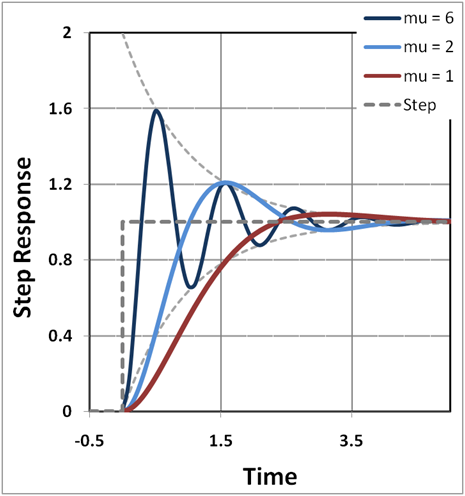
\includegraphics[height=8cm]{media/stepresponse_temp}\\
% \end{center}
% \caption{Step response of some system [XXX]}
% \label{stepresponsefig}
% \end{figure}
